\documentclass[12pt]{article}

%packages
%\usepackage{latexsym}
\usepackage{graphicx}
\usepackage{color}
\usepackage{amsmath}
\usepackage{dsfont}
\usepackage{placeins}
\usepackage{amssymb}
\usepackage{wasysym}
\usepackage{abstract}
\usepackage{hyperref}
\usepackage{etoolbox}
\usepackage{datetime}
\usepackage{xcolor}
\usepackage{alphalph}
\settimeformat{ampmtime}

%\usepackage{pstricks,pst-node,pst-tree}

%\usepackage{algpseudocode}
%\usepackage{amsthm}
%\usepackage{hyperref}
%\usepackage{mathrsfs}
%\usepackage{amsfonts}
%\usepackage{bbding}
%\usepackage{listings}
%\usepackage{appendix}
\usepackage[margin=1in]{geometry}
%\geometry{papersize={8.5in,11in},total={6.5in,9in}}
%\usepackage{cancel}
%\usepackage{algorithmic, algorithm}

\makeatletter
\def\maxwidth{ %
  \ifdim\Gin@nat@width>\linewidth
    \linewidth
  \else
    \Gin@nat@width
  \fi
}
\makeatother

\definecolor{fgcolor}{rgb}{0.345, 0.345, 0.345}
\newcommand{\hlnum}[1]{\textcolor[rgb]{0.686,0.059,0.569}{#1}}%
\newcommand{\hlstr}[1]{\textcolor[rgb]{0.192,0.494,0.8}{#1}}%
\newcommand{\hlcom}[1]{\textcolor[rgb]{0.678,0.584,0.686}{\textit{#1}}}%
\newcommand{\hlopt}[1]{\textcolor[rgb]{0,0,0}{#1}}%
\newcommand{\hlstd}[1]{\textcolor[rgb]{0.345,0.345,0.345}{#1}}%
\newcommand{\hlkwa}[1]{\textcolor[rgb]{0.161,0.373,0.58}{\textbf{#1}}}%
\newcommand{\hlkwb}[1]{\textcolor[rgb]{0.69,0.353,0.396}{#1}}%
\newcommand{\hlkwc}[1]{\textcolor[rgb]{0.333,0.667,0.333}{#1}}%
\newcommand{\hlkwd}[1]{\textcolor[rgb]{0.737,0.353,0.396}{\textbf{#1}}}%

\usepackage{framed}
\makeatletter
\newenvironment{kframe}{%
 \def\at@end@of@kframe{}%
 \ifinner\ifhmode%
  \def\at@end@of@kframe{\end{minipage}}%
  \begin{minipage}{\columnwidth}%
 \fi\fi%
 \def\FrameCommand##1{\hskip\@totalleftmargin \hskip-\fboxsep
 \colorbox{shadecolor}{##1}\hskip-\fboxsep
     % There is no \\@totalrightmargin, so:
     \hskip-\linewidth \hskip-\@totalleftmargin \hskip\columnwidth}%
 \MakeFramed {\advance\hsize-\width
   \@totalleftmargin\z@ \linewidth\hsize
   \@setminipage}}%
 {\par\unskip\endMakeFramed%
 \at@end@of@kframe}
\makeatother

\definecolor{shadecolor}{rgb}{.77, .77, .77}
\definecolor{messagecolor}{rgb}{0, 0, 0}
\definecolor{warningcolor}{rgb}{1, 0, 1}
\definecolor{errorcolor}{rgb}{1, 0, 0}
\newenvironment{knitrout}{}{} % an empty environment to be redefined in TeX

\usepackage{alltt}
\usepackage[T1]{fontenc}

\newcommand{\qu}[1]{``#1''}
\newcounter{probnum}
\setcounter{probnum}{1}

%create definition to allow local margin changes
\def\changemargin#1#2{\list{}{\rightmargin#2\leftmargin#1}\item[]}
\let\endchangemargin=\endlist 

%allow equations to span multiple pages
\allowdisplaybreaks

%define colors and color typesetting conveniences
\definecolor{gray}{rgb}{0.5,0.5,0.5}
\definecolor{black}{rgb}{0,0,0}
\definecolor{white}{rgb}{1,1,1}
\definecolor{blue}{rgb}{0.5,0.5,1}
\newcommand{\inblue}[1]{\color{blue}#1 \color{black}}
\definecolor{green}{rgb}{0.133,0.545,0.133}
\newcommand{\ingreen}[1]{\color{green}#1 \color{black}}
\definecolor{yellow}{rgb}{1,1,0}
\newcommand{\inyellow}[1]{\color{yellow}#1 \color{black}}
\definecolor{orange}{rgb}{0.9,0.649,0}
\newcommand{\inorange}[1]{\color{orange}#1 \color{black}}
\definecolor{red}{rgb}{1,0.133,0.133}
\newcommand{\inred}[1]{\color{red}#1 \color{black}}
\definecolor{purple}{rgb}{0.58,0,0.827}
\newcommand{\inpurple}[1]{\color{purple}#1 \color{black}}
\definecolor{backgcode}{rgb}{0.97,0.97,0.8}
\definecolor{Brown}{cmyk}{0,0.81,1,0.60}
\definecolor{OliveGreen}{cmyk}{0.64,0,0.95,0.40}
\definecolor{CadetBlue}{cmyk}{0.62,0.57,0.23,0}

%define new math operators
\DeclareMathOperator*{\argmax}{arg\,max~}
\DeclareMathOperator*{\argmin}{arg\,min~}
\DeclareMathOperator*{\argsup}{arg\,sup~}
\DeclareMathOperator*{\arginf}{arg\,inf~}
\DeclareMathOperator*{\convolution}{\text{\Huge{$\ast$}}}
\newcommand{\infconv}[2]{\convolution^\infty_{#1 = 1} #2}
%true functions

%%%% GENERAL SHORTCUTS

%shortcuts for pure typesetting conveniences
\newcommand{\bv}[1]{\boldsymbol{#1}}

%shortcuts for compound constants
\newcommand{\BetaDistrConst}{\dfrac{\Gamma(\alpha + \beta)}{\Gamma(\alpha)\Gamma(\beta)}}
\newcommand{\NormDistrConst}{\dfrac{1}{\sqrt{2\pi\sigma^2}}}

%shortcuts for conventional symbols
\newcommand{\tsq}{\tau^2}
\newcommand{\tsqh}{\hat{\tau}^2}
\newcommand{\sigsq}{\sigma^2}
\newcommand{\sigsqsq}{\parens{\sigma^2}^2}
\newcommand{\sigsqovern}{\dfrac{\sigsq}{n}}
\newcommand{\tausq}{\tau^2}
\newcommand{\tausqalpha}{\tau^2_\alpha}
\newcommand{\tausqbeta}{\tau^2_\beta}
\newcommand{\tausqsigma}{\tau^2_\sigma}
\newcommand{\betasq}{\beta^2}
\newcommand{\sigsqvec}{\bv{\sigma}^2}
\newcommand{\sigsqhat}{\hat{\sigma}^2}
\newcommand{\sigsqhatmlebayes}{\sigsqhat_{\text{Bayes, MLE}}}
\newcommand{\sigsqhatmle}[1]{\sigsqhat_{#1, \text{MLE}}}
\newcommand{\bSigma}{\bv{\Sigma}}
\newcommand{\bSigmainv}{\bSigma^{-1}}
\newcommand{\thetavec}{\bv{\theta}}
\newcommand{\thetahat}{\hat{\theta}}
\usepackage{accents}
\newlength{\dhatheight}
\newcommand{\doublehat}[1]{%
    \settoheight{\dhatheight}{\ensuremath{\hat{#1}}}%
    \addtolength{\dhatheight}{-0.35ex}%
    \hat{\vphantom{\rule{1pt}{\dhatheight}}%
    \smash{\hat{#1}}}}

\newcommand{\thetahathat}{\doublehat{\theta}}
\newcommand{\thetahatmle}{\hat{\theta}_{\mathrm{MLE}}}
\newcommand{\thetavechatmle}{\hat{\thetavec}_{\mathrm{MLE}}}
\newcommand{\muhat}{\hat{\mu}}
\newcommand{\musq}{\mu^2}
\newcommand{\muvec}{\bv{\mu}}
\newcommand{\muhatmle}{\muhat_{\text{MLE}}}
\newcommand{\lambdahat}{\hat{\lambda}}
\newcommand{\lambdahatmle}{\lambdahat_{\text{MLE}}}
\newcommand{\etavec}{\bv{\eta}}
\newcommand{\alphavec}{\bv{\alpha}}
\newcommand{\minimaxdec}{\delta^*_{\mathrm{mm}}}
\newcommand{\ybar}{\bar{y}}
\newcommand{\xbar}{\bar{x}}
\newcommand{\Xbar}{\bar{X}}
\newcommand{\phat}{\hat{p}}
\newcommand{\Phat}{\hat{P}}
\newcommand{\Zbar}{\bar{Z}}
\newcommand{\iid}{~{\buildrel iid \over \sim}~}
\newcommand{\inddist}{~{\buildrel ind \over \sim}~}
\newcommand{\approxdist}{~{\buildrel approx \over \sim}~}
\newcommand{\equalsindist}{~{\buildrel d \over =}~}
\newcommand{\loglik}[1]{\ell\parens{#1}}
\newcommand{\thetahatkminone}{\thetahat^{(k-1)}}
\newcommand{\thetahatkplusone}{\thetahat^{(k+1)}}
\newcommand{\thetahatk}{\thetahat^{(k)}}
\newcommand{\half}{\frac{1}{2}}
\newcommand{\third}{\frac{1}{3}}
\newcommand{\twothirds}{\frac{2}{3}}
\newcommand{\fourth}{\frac{1}{4}}
\newcommand{\fifth}{\frac{1}{5}}
\newcommand{\sixth}{\frac{1}{6}}

%shortcuts for vector and matrix notation
\newcommand{\A}{\bv{A}}
\newcommand{\At}{\A^T}
\newcommand{\Ainv}{\inverse{\A}}
\newcommand{\B}{\bv{B}}
\newcommand{\K}{\bv{K}}
\newcommand{\Kt}{\K^T}
\newcommand{\Kinv}{\inverse{K}}
\newcommand{\Kinvt}{(\Kinv)^T}
\newcommand{\M}{\bv{M}}
\newcommand{\Bt}{\B^T}
\newcommand{\Q}{\bv{Q}}
\newcommand{\Qt}{\Q^T}
\newcommand{\R}{\bv{R}}
\newcommand{\Rt}{\R^T}
\newcommand{\Z}{\bv{Z}}
\newcommand{\X}{\bv{X}}
\newcommand{\Xsub}{\X_{\text{(sub)}}}
\newcommand{\Xsubadj}{\X_{\text{(sub,adj)}}}
\newcommand{\I}{\bv{I}}
\newcommand{\Y}{\bv{Y}}
\newcommand{\T}{\bv{T}}
\newcommand{\sigsqI}{\sigsq\I}
\renewcommand{\P}{\bv{P}}
\newcommand{\Psub}{\P_{\text{(sub)}}}
\newcommand{\Pt}{\P^T}
\newcommand{\Pii}{P_{ii}}
\newcommand{\Pij}{P_{ij}}
\newcommand{\IminP}{(\I-\P)}
\newcommand{\Xt}{\bv{X}^T}
\newcommand{\XtX}{\Xt\X}
\newcommand{\XtXinv}{\parens{\Xt\X}^{-1}}
\newcommand{\XtXinvXt}{\XtXinv\Xt}
\newcommand{\XXtXinvXt}{\X\XtXinvXt}
\newcommand{\x}{\bv{x}}
\newcommand{\p}{\bv{p}}
\newcommand{\onevec}{\bv{1}}
\newcommand{\oneton}{1, \ldots, n}
\newcommand{\yoneton}{y_1, \ldots, y_n}
\newcommand{\yonetonorder}{y_{(1)}, \ldots, y_{(n)}}
\newcommand{\Yoneton}{Y_1, \ldots, Y_n}
\newcommand{\iinoneton}{i \in \braces{\oneton}}
\newcommand{\onetom}{1, \ldots, m}
\newcommand{\jinonetom}{j \in \braces{\onetom}}
\newcommand{\xoneton}{x_1, \ldots, x_n}
\newcommand{\Xoneton}{X_1, \ldots, X_n}
\newcommand{\xt}{\x^T}
\newcommand{\y}{\bv{y}}
\newcommand{\yt}{\y^T}
\renewcommand{\c}{\bv{c}}
\newcommand{\ct}{\c^T}
\newcommand{\tstar}{\bv{t}^*}
\renewcommand{\u}{\bv{u}}
\renewcommand{\v}{\bv{v}}
\renewcommand{\a}{\bv{a}}
\newcommand{\s}{\bv{s}}
\newcommand{\yadj}{\y_{\text{(adj)}}}
\newcommand{\xjadj}{\x_{j\text{(adj)}}}
\newcommand{\xjadjM}{\x_{j \perp M}}
\newcommand{\yhat}{\hat{\y}}
\newcommand{\yhatsub}{\yhat_{\text{(sub)}}}
\newcommand{\yhatstar}{\yhat^*}
\newcommand{\yhatstarnew}{\yhatstar_{\text{new}}}
\newcommand{\z}{\bv{z}}
\newcommand{\zt}{\z^T}
\newcommand{\bb}{\bv{b}}
\newcommand{\bbt}{\bb^T}
\newcommand{\bbeta}{\bv{\beta}}
\newcommand{\beps}{\bv{\epsilon}}
\newcommand{\bepst}{\beps^T}
\newcommand{\e}{\bv{e}}
\newcommand{\Mofy}{\M(\y)}
\newcommand{\KofAlpha}{K(\alpha)}
\newcommand{\ellset}{\mathcal{L}}
\newcommand{\oneminalph}{1-\alpha}
\newcommand{\SSE}{\text{SSE}}
\newcommand{\SSEsub}{\text{SSE}_{\text{(sub)}}}
\newcommand{\MSE}{\text{MSE}}
\newcommand{\RMSE}{\text{RMSE}}
\newcommand{\SSR}{\text{SSR}}
\newcommand{\SST}{\text{SST}}
\newcommand{\JSest}{\delta_{\text{JS}}(\x)}
\newcommand{\Bayesest}{\delta_{\text{Bayes}}(\x)}
\newcommand{\EmpBayesest}{\delta_{\text{EmpBayes}}(\x)}
\newcommand{\BLUPest}{\delta_{\text{BLUP}}}
\newcommand{\MLEest}[1]{\hat{#1}_{\text{MLE}}}

%shortcuts for Linear Algebra stuff (i.e. vectors and matrices)
\newcommand{\twovec}[2]{\bracks{\begin{array}{c} #1 \\ #2 \end{array}}}
\newcommand{\threevec}[3]{\bracks{\begin{array}{c} #1 \\ #2 \\ #3 \end{array}}}
\newcommand{\fivevec}[5]{\bracks{\begin{array}{c} #1 \\ #2 \\ #3 \\ #4 \\ #5 \end{array}}}
\newcommand{\twobytwomat}[4]{\bracks{\begin{array}{cc} #1 & #2 \\ #3 & #4 \end{array}}}
\newcommand{\threebytwomat}[6]{\bracks{\begin{array}{cc} #1 & #2 \\ #3 & #4 \\ #5 & #6 \end{array}}}

%shortcuts for conventional compound symbols
\newcommand{\thetainthetas}{\theta \in \Theta}
\newcommand{\reals}{\mathbb{R}}
\newcommand{\complexes}{\mathbb{C}}
\newcommand{\rationals}{\mathbb{Q}}
\newcommand{\integers}{\mathbb{Z}}
\newcommand{\naturals}{\mathbb{N}}
\newcommand{\forallninN}{~~\forall n \in \naturals}
\newcommand{\forallxinN}[1]{~~\forall #1 \in \reals}
\newcommand{\matrixdims}[2]{\in \reals^{\,#1 \times #2}}
\newcommand{\inRn}[1]{\in \reals^{\,#1}}
\newcommand{\mathimplies}{\quad\Rightarrow\quad}
\newcommand{\mathlogicequiv}{\quad\Leftrightarrow\quad}
\newcommand{\eqncomment}[1]{\quad \text{(#1)}}
\newcommand{\limitn}{\lim_{n \rightarrow \infty}}
\newcommand{\limitN}{\lim_{N \rightarrow \infty}}
\newcommand{\limitd}{\lim_{d \rightarrow \infty}}
\newcommand{\limitt}{\lim_{t \rightarrow \infty}}
\newcommand{\limitsupn}{\limsup_{n \rightarrow \infty}~}
\newcommand{\limitinfn}{\liminf_{n \rightarrow \infty}~}
\newcommand{\limitk}{\lim_{k \rightarrow \infty}}
\newcommand{\limsupn}{\limsup_{n \rightarrow \infty}}
\newcommand{\limsupk}{\limsup_{k \rightarrow \infty}}
\newcommand{\floor}[1]{\left\lfloor #1 \right\rfloor}
\newcommand{\ceil}[1]{\left\lceil #1 \right\rceil}

%shortcuts for environments
\newcommand{\beqn}{\vspace{-0.25cm}\begin{eqnarray*}}
\newcommand{\eeqn}{\end{eqnarray*}}
\newcommand{\bneqn}{\vspace{-0.25cm}\begin{eqnarray}}
\newcommand{\eneqn}{\end{eqnarray}}

%shortcuts for mini environments
\newcommand{\parens}[1]{\left(#1\right)}
\newcommand{\squared}[1]{\parens{#1}^2}
\newcommand{\tothepow}[2]{\parens{#1}^{#2}}
\newcommand{\prob}[1]{\mathbb{P}\parens{#1}}
\newcommand{\cprob}[2]{\prob{#1~|~#2}}
\newcommand{\littleo}[1]{o\parens{#1}}
\newcommand{\bigo}[1]{O\parens{#1}}
\newcommand{\Lp}[1]{\mathbb{L}^{#1}}
\renewcommand{\arcsin}[1]{\text{arcsin}\parens{#1}}
\newcommand{\prodonen}[2]{\bracks{\prod_{#1=1}^n #2}}
\newcommand{\mysum}[4]{\sum_{#1=#2}^{#3} #4}
\newcommand{\sumonen}[2]{\sum_{#1=1}^n #2}
\newcommand{\infsum}[2]{\sum_{#1=1}^\infty #2}
\newcommand{\infprod}[2]{\prod_{#1=1}^\infty #2}
\newcommand{\infunion}[2]{\bigcup_{#1=1}^\infty #2}
\newcommand{\infinter}[2]{\bigcap_{#1=1}^\infty #2}
\newcommand{\infintegral}[2]{\int^\infty_{-\infty} #2 ~\text{d}#1}
\newcommand{\supthetas}[1]{\sup_{\thetainthetas}\braces{#1}}
\newcommand{\bracks}[1]{\left[#1\right]}
\newcommand{\braces}[1]{\left\{#1\right\}}
\newcommand{\set}[1]{\left\{#1\right\}}
\newcommand{\abss}[1]{\left|#1\right|}
\newcommand{\norm}[1]{\left|\left|#1\right|\right|}
\newcommand{\normsq}[1]{\norm{#1}^2}
\newcommand{\inverse}[1]{\parens{#1}^{-1}}
\newcommand{\rowof}[2]{\parens{#1}_{#2\cdot}}

%shortcuts for functionals
\newcommand{\realcomp}[1]{\text{Re}\bracks{#1}}
\newcommand{\imagcomp}[1]{\text{Im}\bracks{#1}}
\newcommand{\range}[1]{\text{range}\bracks{#1}}
\newcommand{\colsp}[1]{\text{colsp}\bracks{#1}}
\newcommand{\rowsp}[1]{\text{rowsp}\bracks{#1}}
\newcommand{\tr}[1]{\text{tr}\bracks{#1}}
\newcommand{\rank}[1]{\text{rank}\bracks{#1}}
\newcommand{\proj}[2]{\text{Proj}_{#1}\bracks{#2}}
\newcommand{\projcolspX}[1]{\text{Proj}_{\colsp{\X}}\bracks{#1}}
\newcommand{\median}[1]{\text{median}\bracks{#1}}
\newcommand{\mean}[1]{\text{mean}\bracks{#1}}
\newcommand{\dime}[1]{\text{dim}\bracks{#1}}
\renewcommand{\det}[1]{\text{det}\bracks{#1}}
\newcommand{\expe}[1]{\mathbb{E}\bracks{#1}}
\newcommand{\expeabs}[1]{\expe{\abss{#1}}}
\newcommand{\expesub}[2]{\mathbb{E}_{#1}\bracks{#2}}
\newcommand{\indic}[1]{\mathds{1}_{#1}}
\newcommand{\var}[1]{\mathbb{V}\text{ar}\bracks{#1}}
\newcommand{\cov}[2]{\mathbb{C}\text{ov}\bracks{#1, #2}}
\newcommand{\corrtwo}[2]{\text{Corr}\bracks{#1, #2}}
\newcommand{\corr}[1]{\text{Corr}\bracks{#1}}
\newcommand{\se}[1]{\mathbb{S}\text{E}\bracks{#1}}
\newcommand{\seest}[1]{\hat{\mathbb{S}\text{E}}\bracks{#1}}
\newcommand{\bias}[1]{\text{Bias}\bracks{#1}}
\newcommand{\derivop}[2]{\dfrac{\text{d}}{\text{d} #1}\bracks{#2}}
\newcommand{\partialop}[2]{\dfrac{\partial}{\partial #1}\bracks{#2}}
\newcommand{\secpartialop}[2]{\dfrac{\partial^2}{\partial #1^2}\bracks{#2}}
\newcommand{\mixpartialop}[3]{\dfrac{\partial^2}{\partial #1 \partial #2}\bracks{#3}}

%shortcuts for functions
\renewcommand{\exp}[1]{\mathrm{exp}\parens{#1}}
\renewcommand{\cos}[1]{\text{cos}\parens{#1}}
\renewcommand{\sin}[1]{\text{sin}\parens{#1}}
\newcommand{\sign}[1]{\text{sign}\parens{#1}}
\newcommand{\are}[1]{\mathrm{ARE}\parens{#1}}
\newcommand{\natlog}[1]{\ln\parens{#1}}
\newcommand{\oneover}[1]{\frac{1}{#1}}
\newcommand{\overtwo}[1]{\frac{#1}{2}}
\newcommand{\overn}[1]{\frac{#1}{n}}
\newcommand{\oneoversqrt}[1]{\oneover{\sqrt{#1}}}
\newcommand{\sqd}[1]{\parens{#1}^2}
\newcommand{\loss}[1]{\ell\parens{\theta, #1}}
\newcommand{\losstwo}[2]{\ell\parens{#1, #2}}
\newcommand{\cf}{\phi(t)}

%English language specific shortcuts
\newcommand{\ie}{\textit{i.e.} }
\newcommand{\AKA}{\textit{AKA} }
\renewcommand{\iff}{\textit{iff}}
\newcommand{\eg}{\textit{e.g.} }
\newcommand{\st}{\textit{s.t.} }
\newcommand{\wrt}{\textit{w.r.t.} }
\newcommand{\mathst}{~~\text{\st}~~}
\newcommand{\mathand}{~~\text{and}~~}
\newcommand{\ala}{\textit{a la} }
\newcommand{\ppp}{posterior predictive p-value}
\newcommand{\dd}{dataset-to-dataset}

%shortcuts for distribution titles
\newcommand{\logistic}[2]{\mathrm{Logistic}\parens{#1,\,#2}}
\newcommand{\bernoulli}[1]{\mathrm{Bern}\parens{#1}}
\newcommand{\betanot}[2]{\mathrm{Beta}\parens{#1,\,#2}}
\newcommand{\stdbetanot}{\betanot{\alpha}{\beta}}
\newcommand{\multnormnot}[3]{\mathcal{N}_{#1}\parens{#2,\,#3}}
\newcommand{\normnot}[2]{\mathcal{N}\parens{#1,\,#2}}
\newcommand{\classicnormnot}{\normnot{\mu}{\sigsq}}
\newcommand{\stdnormnot}{\normnot{0}{1}}
\newcommand{\uniformdiscrete}[1]{\mathrm{Uniform}\parens{\braces{#1}}}
\newcommand{\uniform}[2]{\mathrm{U}\parens{#1,\,#2}}
\newcommand{\stduniform}{\uniform{0}{1}}
\newcommand{\geometric}[1]{\mathrm{Geometric}\parens{#1}}
\newcommand{\hypergeometric}[3]{\mathrm{Hypergeometric}\parens{#1,\,#2,\,#3}}
\newcommand{\exponential}[1]{\mathrm{Exp}\parens{#1}}
\newcommand{\gammadist}[2]{\mathrm{Gamma}\parens{#1, #2}}
\newcommand{\poisson}[1]{\mathrm{Poisson}\parens{#1}}
\newcommand{\binomial}[2]{\mathrm{Binomial}\parens{#1,\,#2}}
\newcommand{\negbin}[2]{\mathrm{NegBin}\parens{#1,\,#2}}
\newcommand{\rayleigh}[1]{\mathrm{Rayleigh}\parens{#1}}
\newcommand{\multinomial}[2]{\mathrm{Multinomial}\parens{#1,\,#2}}
\newcommand{\gammanot}[2]{\mathrm{Gamma}\parens{#1,\,#2}}
\newcommand{\cauchynot}[2]{\text{Cauchy}\parens{#1,\,#2}}
\newcommand{\invchisqnot}[1]{\text{Inv}\chisq{#1}}
\newcommand{\invscaledchisqnot}[2]{\text{ScaledInv}\ncchisq{#1}{#2}}
\newcommand{\invgammanot}[2]{\text{InvGamma}\parens{#1,\,#2}}
\newcommand{\chisq}[1]{\chi^2_{#1}}
\newcommand{\ncchisq}[2]{\chi^2_{#1}\parens{#2}}
\newcommand{\ncF}[3]{F_{#1,#2}\parens{#3}}

%shortcuts for PDF's of common distributions
\newcommand{\logisticpdf}[3]{\oneover{#3}\dfrac{\exp{-\dfrac{#1 - #2}{#3}}}{\parens{1+\exp{-\dfrac{#1 - #2}{#3}}}^2}}
\newcommand{\betapdf}[3]{\dfrac{\Gamma(#2 + #3)}{\Gamma(#2)\Gamma(#3)}#1^{#2-1} (1-#1)^{#3-1}}
\newcommand{\normpdf}[3]{\frac{1}{\sqrt{2\pi#3}}\exp{-\frac{1}{2#3}(#1 - #2)^2}}
\newcommand{\normpdfvarone}[2]{\dfrac{1}{\sqrt{2\pi}}e^{-\half(#1 - #2)^2}}
\newcommand{\chisqpdf}[2]{\dfrac{1}{2^{#2/2}\Gamma(#2/2)}\; {#1}^{#2/2-1} e^{-#1/2}}
\newcommand{\invchisqpdf}[2]{\dfrac{2^{-\overtwo{#1}}}{\Gamma(#2/2)}\,{#1}^{-\overtwo{#2}-1}  e^{-\oneover{2 #1}}}
\newcommand{\exponentialpdf}[2]{#2\exp{-#2#1}}
\newcommand{\poissonpdf}[2]{\dfrac{e^{-#1} #1^{#2}}{#2!}}
\newcommand{\binomialpdf}[3]{\binom{#2}{#1}#3^{#1}(1-#3)^{#2-#1}}
\newcommand{\rayleighpdf}[2]{\dfrac{#1}{#2^2}\exp{-\dfrac{#1^2}{2 #2^2}}}
\newcommand{\gammapdf}[3]{\dfrac{#3^#2}{\Gamma\parens{#2}}#1^{#2-1}\exp{-#3 #1}}
\newcommand{\cauchypdf}[3]{\oneover{\pi} \dfrac{#3}{\parens{#1-#2}^2 + #3^2}}
\newcommand{\Gammaf}[1]{\Gamma\parens{#1}}

%shortcuts for miscellaneous typesetting conveniences
\newcommand{\notesref}[1]{\marginpar{\color{gray}\tt #1\color{black}}}

%%%% DOMAIN-SPECIFIC SHORTCUTS

%Real analysis related shortcuts
\newcommand{\zeroonecl}{\bracks{0,1}}
\newcommand{\forallepsgrzero}{\forall \epsilon > 0~~}
\newcommand{\lessthaneps}{< \epsilon}
\newcommand{\fraccomp}[1]{\text{frac}\bracks{#1}}

%Bayesian related shortcuts
\newcommand{\yrep}{y^{\text{rep}}}
\newcommand{\yrepisq}{(\yrep_i)^2}
\newcommand{\yrepvec}{\bv{y}^{\text{rep}}}


%Probability shortcuts
\newcommand{\SigField}{\mathcal{F}}
\newcommand{\ProbMap}{\mathcal{P}}
\newcommand{\probtrinity}{\parens{\Omega, \SigField, \ProbMap}}
\newcommand{\convp}{~{\buildrel p \over \rightarrow}~}
\newcommand{\convLp}[1]{~{\buildrel \Lp{#1} \over \rightarrow}~}
\newcommand{\nconvp}{~{\buildrel p \over \nrightarrow}~}
\newcommand{\convae}{~{\buildrel a.e. \over \longrightarrow}~}
\newcommand{\convau}{~{\buildrel a.u. \over \longrightarrow}~}
\newcommand{\nconvau}{~{\buildrel a.u. \over \nrightarrow}~}
\newcommand{\nconvae}{~{\buildrel a.e. \over \nrightarrow}~}
\newcommand{\convd}{~{\buildrel \mathcal{D} \over \rightarrow}~}
\newcommand{\nconvd}{~{\buildrel \mathcal{D} \over \nrightarrow}~}
\newcommand{\withprob}{~~\text{w.p.}~~}
\newcommand{\io}{~~\text{i.o.}}

\newcommand{\Acl}{\bar{A}}
\newcommand{\ENcl}{\bar{E}_N}
\newcommand{\diam}[1]{\text{diam}\parens{#1}}

\newcommand{\taua}{\tau_a}

\newcommand{\myint}[4]{\int_{#2}^{#3} #4 \,\text{d}#1}
\newcommand{\laplacet}[1]{\mathscr{L}\bracks{#1}}
\newcommand{\laplaceinvt}[1]{\mathscr{L}^{-1}\bracks{#1}}
\renewcommand{\min}[1]{\text{min}\braces{#1}}
\renewcommand{\max}[1]{\text{max}\braces{#1}}

\newcommand{\Vbar}[1]{\bar{V}\parens{#1}}
\newcommand{\expnegrtau}{\exp{-r\tau}}

%%% problem typesetting
\definecolor{darkgrey}{rgb}{0.10,0.10,0.9}

\newcommand{\problem}[1]{\noindent \colorbox{black}{{\color{yellow} \large{\textsf{\textbf{Problem \arabic{probnum}}}}~}} \addtocounter{probnum}{1} \vspace{0.2cm} \\ \iftoggle{professormode}{}{\color{darkgrey}} #1}

\newcommand{\easysubproblem}[1]{\ingreen{\item} \iftoggle{professormode}{}{\color{darkgrey}} [easy] #1 \color{black} }
\newcommand{\intermediatesubproblem}[1]{\inorange{\item} \iftoggle{professormode}{}{\color{darkgrey}} [harder] #1 \color{black} }
\newcommand{\hardsubproblem}[1]{\inred{\item} \iftoggle{professormode}{}{\color{darkgrey}} [difficult] #1 \color{black} }
\newcommand{\extracreditsubproblem}[1]{\inpurple{\item} \iftoggle{professormode}{}{\color{darkgrey}} [E.C.] #1 \color{black} }


\newcommand{\spc}[1]{\iftoggle{professormode}{\\ \vspace{#1cm}}{\\ \vspace{-0.3cm}}}

\makeatletter
\newalphalph{\alphmult}[mult]{\@alph}{26}
\renewcommand{\labelenumi}{(\alphmult{\value{enumi}})}

\newcommand{\support}[1]{\text{Supp}\bracks{#1}}
\newcommand{\mode}[1]{\text{Mode}\bracks{#1}}
\newcommand{\IQR}[1]{\text{IQR}\bracks{#1}}
\newcommand{\quantile}[2]{\text{Quantile}\bracks{#1,\,#2}}


\newtoggle{professormode}
\toggletrue{professormode} %STUDENTS: DELETE or COMMENT this line



\title{MATH 369/650 Fall \the\year{} Homework \#4}

\author{Professor Adam Kapelner} %STUDENTS: write your name here

\iftoggle{professormode}{
\date{Due by email 11:59PM Saturday, October 24, \the\year{} \\ \vspace{0.5cm} \small (this document last updated \today ~at \currenttime)}
}

\renewcommand{\abstractname}{Instructions and Philosophy}

\begin{document}
\maketitle

\iftoggle{professormode}{
\begin{abstract}
The path to success in this class is to do many problems. Unlike other courses, exclusively doing reading(s) will not help. Coming to lecture is akin to watching workout videos; thinking about and solving problems on your own is the actual ``working out.''  Feel free to \qu{work out} with others; \textbf{I want you to work on this in groups.}

Reading is still \textit{required}. For this homework set, review Math 241 concerning the normal distribution. Then read about the class topics (e.g. CRLB, Fisher Information, asymptotically normal estimators, etc) in the two recommended textbooks and online.

The problems below are color coded: \ingreen{green} problems are considered \textit{easy} and marked \qu{[easy]}; \inorange{yellow} problems are considered \textit{intermediate} and marked \qu{[harder]}, \inred{red} problems are considered \textit{difficult} and marked \qu{[difficult]} and \inpurple{purple} problems are extra credit. The \textit{easy} problems are intended to be ``giveaways'' if you went to class. Do as much as you can of the others; I expect you to at least attempt the \textit{difficult} problems. \qu{[MA]} are for those registered for the 600-level class and extra credit otherwise.

This homework is worth 100 points but the point distribution will not be determined until after the due date. See syllabus for the policy on late homework.

Up to 7 points are given as a bonus if the homework is typed using \LaTeX. Links to instaling \LaTeX~and program for compiling \LaTeX~is found on the syllabus. You are encouraged to use \url{overleaf.com}. If you are handing in homework this way, read the comments in the code; there are two lines to comment out and you should replace my name with yours and write your section. The easiest way to use overleaf is to copy the raw text from hwxx.tex and preamble.tex into two new overleaf tex files with the same name. If you are asked to make drawings, you can take a picture of your handwritten drawing and insert them as figures or leave space using the \qu{$\backslash$vspace} command and draw them in after printing or attach them stapled.

The document is available with spaces for you to write your answers. If not using \LaTeX, print this document and write in your answers. I do not accept homeworks which are \textit{not} on this printout. Keep this first page printed for your records.

\end{abstract}

\thispagestyle{empty}
\vspace{1cm}
NAME: \line(1,0){380}
\clearpage
}


\problem{We will prove the CRLB and some other facts here.}


\begin{enumerate}


\easysubproblem{Prove the CRLB from scratch. Justify each step.}\spc{22}

\easysubproblem{State Thm 5.5.4 p233 C\&B.}\spc{1}

\easysubproblem{Use Thm 5.5.4 to prove that if $X \convp c$ then $\frac{X}{c} \convp 1$ and $\frac{c}{X} \convp 1$.}\spc{1}

\easysubproblem{State Slutsky's Theorem.}\spc{1}

\hardsubproblem{Assume an iid DGP with mean $\theta$ and variance $\sigsq$. Recall the CLT,

\beqn
\frac{\Xbar - \theta}{\frac{\sigma}{\sqrt{n}}} \convd \stdnormnot.
\eeqn

Let $S^2$ be the estimator for $\sigsq$ we discussed in class. In a more advanced probability class, you can show that $S \convp \sigma$. Use Thm 5.5.4 and Slutsky's Theorem to show that the usual t statistic is asymptotically normal i.e. prove that

\beqn
\frac{\Xbar - \theta}{\frac{S}{\sqrt{n}}} \convd \stdnormnot
\eeqn

Hint: it is two steps. Don't overthink it!}\spc{10}

\easysubproblem{Prove that the MLE is asymptotically normal and asymptotically efficient from scratch. Justify each step.}\spc{22}


\hardsubproblem{Prove that the score function is asymptotically normal using the CLT. The facts should be found in the previous problem which you got from the notes.}\spc{6}


\hardsubproblem{Prove that Fisher Information which is defined as $I(\theta) := \expe{\ell'(\theta; X)}$ is equal to $\expe{\ell''(\theta; X)}$. If you make any assumptions proving this, indicate it so. This is not easy. There will be lots of hints on slack given.}\spc{16}

\end{enumerate}


\problem{We will get practice finding MLE's, their asymptotic distributions and proving estimators are UMVUE's.}


\begin{enumerate}


\easysubproblem{Consider the DGP $\Xoneton \iid \bernoulli{\theta}$.  Find $\thetahatmle$.}\spc{6}


\easysubproblem{Prove that the MLE is the UMVUE for $\theta$.}\spc{6}


\easysubproblem{Write the approximate distribution of the MLE.}\spc{10}


%\easysubproblem{Consider the DGP $\Xoneton \iid \normnot{\theta_1}{\theta_2}$. Find $\thetahatmle_1$.}\spc{5}
%
%
%\easysubproblem{Prove that the MLE is the UMVUE for $\theta_1$.}\spc{6}
%
%\easysubproblem{Write the approximate distribution of the MLE.}\spc{1}

\intermediatesubproblem{Consider the DGP $\Xoneton \iid \normnot{0}{\theta}$. Find $\thetahatmle$.}\spc{6}

\intermediatesubproblem{Prove that the MLE is the UMVUE for $\theta$.}\spc{6}

\easysubproblem{Write the approximate distribution of the MLE.}\spc{1}


\intermediatesubproblem{Consider the DGP $\Xoneton \iid \poisson{\theta} := \theta^x e^{-\theta} / x!$ where $\expe{X} = \theta$ and $\var{X} = \theta$. Find $\thetahatmle$.}\spc{6}

\easysubproblem{Prove that the MLE is the UMVUE for $\theta$.}\spc{6}

\easysubproblem{Write the approximate distribution of the MLE.}\spc{2}


\hardsubproblem{Consider the DGP $\Xoneton \iid \lognormnot{\theta}{1} := \oneover{x\sqrt{2\pi}} e^{-\half \squared{\natlog{x} - \theta}}$ and find $\thetahatmle$.}\spc{8}

\intermediatesubproblem{Write the approximate distribution of the MLE.}\spc{8}


\hardsubproblem{Consider the DGP $\Xoneton \iid \text{Gumbel}(\theta, 1) := e^{-(x - \theta) - e^{-(x - \theta)}}$ and find $\thetahatmle$.}\spc{9}

\hardsubproblem{Write the approximate distribution of the MLE. You will need the following fact from Math 368 to find the answer: $\expe{e^{-X}} = e^{-\theta}$.}\spc{11}


\hardsubproblem{Consider the DGP $\Xoneton \iid \text{Logistic}(\theta, 1) := e^{-(x - \theta)} / (1 + e^{-(x - \theta)})$. Find an expression for when solved will find $\thetahatmle$. There is no closed form expression that exists.}\spc{9}

\intermediatesubproblem{In a few sentences, explain why it would be difficult to provide the approximate distribution of the MLE.}\spc{6}
\end{enumerate}




\end{document}

\problem{In lecture 6-7, we did two-sided two-sample z and t tests. We will repeat these tests now but do them one sided. For extra practice, I will make them left-sided. To do this, I will switch the indexing of the two populations. The female population is now considered population \#1 and the male population is now considered population \#2. We assume the DGP for female height measurements is $\iid \normnot{\theta_1}{\sigsq_1}$ independent of the DGP for male height measurements assumed to be $\iid \normnot{\theta_2}{\sigsq_2}$. 

The sample sizes, point estimates for the mean and point estimates for the variance computed from the in-class student survey are:

%
%\begin{table}
%\centering
%\begin{tabular}{c|cc}
%& Sample \#1 (Female) & Sample \#2 (Male) \\
%$n$ & 6 & 10 \\
%$\xbar
\beqn
n_1 &=& 6 \\
\xbar_1 &=& 62.3 \\
s^2_1 &=& 2.25^2 \\
n_2 &=& 10 \\
\xbar_2 &=& 70.5 \\
s^2_2 &=& 2.07^2
\eeqn



The theory we wish to prove is that females are shorter than males. We will do so via hypothesis testing at size $\alpha = 5\%$. We will test this under many different assumption scenarios about the variances in the DGP. The results should be approximately the same.}

\begin{enumerate}

\easysubproblem{Write the alternative and null hypotheses. Remember that $\theta_1$ and $\theta_2$ are now switched from class. We will use these hypotheses for the four scenarios in the rest of the problem.}\spc{1}

%%%%%%%%%%%%%%%%%%
\line(1,0){440} \\
We will first assume that the variances are known to be $\sigsq_1 = 3.5^2$ and $\sigsq_2 = 4^2$.

\easysubproblem{Write the exact or approximate distribution of the standardized estimator under the null hypothesis which we denote $(\thetahat_1 - \thetahat_2) / SE~|~H_0$. You should first write the SE as a mathematical expression. Then compute SE to three decimal places. The answer is in lecture 6.}\spc{4}

\easysubproblem{Illustrate the distribution from the previous problem. Label the x-axis and provide tick marks on the x-axis. Leave lots of room on the left side of the x-axis away from the bulk of the sampling distribution!}\spc{8}


\intermediatesubproblem{Will this test be an \emph{exact test} or instead an \emph{approximate test}? Explain.}\spc{3}

\intermediatesubproblem{Compute the retainment region and rejection region (remember $\Theta = \reals$) and denote these two regions in your illustration in (c). To compute these regions, I'll provide you with the following fact: $\Phi(-1.645) = 5\%$ where $\Phi$ is the CDF of the standard normal rv. (These are the kind of facts that will be provided to you on exams).}\spc{2}


\easysubproblem{Why is this test named the \emph{left-sided two-sample z test of unequal variances}?}\spc{3}

\easysubproblem{Run the test and write your conclusion using an English sentence.}\spc{1}

\easysubproblem{What type of error could you have made?}\spc{0}

\intermediatesubproblem{Find the p-value of our estimate as a function of $\Phi$. Illustrate the p-value in the illustration in (c).}\spc{3}

\easysubproblem{Without computing the p-value explicitly, would it be above or below $\alpha = 5\%$? Is the estimate \emph{statistically significant}?}\spc{2}

\hardsubproblem{[MA]  In the general case of  $\theta_{\Delta} := \theta_1 - \theta_2$, $\sigsq_1$, $\sigsq_2$, $n_1$, $n_2$ and $\alpha$, find the power function $POW(\theta_{\Delta}, \sigsq_1, \sigsq_2, n_1, n_2, \alpha)$. }\spc{10}


%%%%%%%%%%%%%%%%%%
\line(1,0){440} \\
We will now assume that the variances are equal and  known to be $\sigsq_1 = \sigsq_2 = \sigsq = 3.76^2$.

\easysubproblem{Write the exact or approximate distribution of the standardized estimator under the null hypothesis which we denote $(\thetahat_1 - \thetahat_2) / SE~|~H_0$. You should first write the SE as a mathematical expression. Then compute SE to three decimal places. The answer is in lecture 6.}\spc{3}

\easysubproblem{Illustrate the distribution from the previous problem. Label the x-axis and provide tick marks on the x-axis. Leave lots of room on the left side of the x-axis away from the bulk of the sampling distribution!}\spc{9}

\intermediatesubproblem{Will this test be an \emph{exact test} or instead an \emph{approximate test}? Explain.}\spc{3}

\intermediatesubproblem{Compute the retainment region and rejection region (remember $\Theta = \reals$) and denote these two regions in your illustration in (m). To compute these regions, I'll provide you with the following fact: $\Phi(-1.645) = 5\%$ where $\Phi$ is the CDF of the standard normal rv. (These are the kind of facts that will be provided to you on exams).}\spc{3}


\easysubproblem{Why is this test named the \emph{left-sided two-sample z test of equal variances}?}\spc{3}

\easysubproblem{Run the test and write your conclusion using an English sentence.}\spc{1}

\easysubproblem{What type of error could you have made?}\spc{0}

\intermediatesubproblem{Find the p-value of our estimate as a function of $\Phi$. Illustrate the p-value in the illustration in (m).}\spc{3}

\easysubproblem{Without computing the p-value explicitly, would it be above or below $\alpha = 5\%$? Is the estimate \emph{statistically significant}?}\spc{2}

%%%%%%%%%%%%%%%%%%
\line(1,0){440} \\
We will now assume that the variances are equal i.e. $\sigsq_1 = \sigsq_2 = \sigsq$ but its value is \emph{unknown}.

\easysubproblem{Write the exact or approximate distribution of the standardized estimator under the null hypothesis which we denote $(\thetahat_1 - \thetahat_2) / SE~|~H_0$. You should first write the SE as a mathematical expression. Then compute SE to three decimal places. The answer is in lecture 6.}\spc{3}

\easysubproblem{Illustrate the distribution from the previous problem. Label the x-axis and provide tick marks on the x-axis. Leave lots of room on the left side of the x-axis away from the bulk of the sampling distribution!}\spc{9}

\intermediatesubproblem{Will this test be an \emph{exact test} or instead an \emph{approximate test}? Explain.}\spc{3}

\intermediatesubproblem{Compute the retainment region and rejection region (remember $\Theta = \reals$) and denote these two regions in your illustration in (v). To compute these regions, I'll provide you with the following fact: $\prob{T_{14} \leq -1.76} = 5\%$ where $T_{14}$ denotes a standard Student's t rv with 14 degrees of freedom. (These are the kind of facts that will be provided to you on exams).}\spc{3}


\easysubproblem{Why is this test named the \emph{left-sided two-sample t test of equal variances}?}\spc{3}

\easysubproblem{Run the test and write your conclusion using an English sentence.}\spc{1}

\easysubproblem{What type of error could you have made?}\spc{0}

\intermediatesubproblem{Find the p-value of our estimate by writing a statement like $\prob{T_{df} < t}$ or $\prob{T_{df} > t}$. You need to solve for $df$, $t$. Illustrate the p-val in the illustration in (v).}\spc{3}

\easysubproblem{Without computing the p-value explicitly, would it be above or below $\alpha = 5\%$? Is the estimate \emph{statistically significant}?}\spc{2}

%%%%%%%%%%%%%%%%%%
\line(1,0){440} \\
We will now assume that the variances are unequal i.e. $\sigsq_1 \neq \sigsq_2$ and both values are \emph{unknown}. This is known as the Behrens-Fisher problem.

\easysubproblem{Write the exact or approximate distribution of the standardized estimator under the null hypothesis which we denote $(\thetahat_1 - \thetahat_2) / SE~|~H_0$. You should first write the SE as a mathematical expression. Then compute SE to three decimal places. The answer is in lecture 7.}\spc{3}

\easysubproblem{Illustrate the distribution from the previous problem. Label the x-axis and provide tick marks on the x-axis. Leave lots of room on the left side of the x-axis away from the bulk of the sampling distribution!}\spc{9}

\intermediatesubproblem{Will this test be an \emph{exact test} or instead an \emph{approximate test}? Explain. (Hint: the exact distribution was solved in 2018 and can be found in \href{https://www.academia.edu/37294681/ON_THE_SOLUTION_OF_A_GENERALIZED_BEHRENS_FISHER_PROBLEM}{this paper}).}\spc{3}

\intermediatesubproblem{Compute the retainment region and rejection region (remember $\Theta = \reals$) and denote these two regions in your illustration in (ee). To compute these regions, I'll provide you with the following fact: $\prob{T_{9.94} \leq -1.81} = 5\%$ where $T_{9.94}$ denotes a standard Student's t rv with 9.94 degrees of freedom. (These are the kind of facts that will be provided to you on exams).}\spc{2}


\easysubproblem{Why is this test named the \emph{left-sided two-sample t test of unequal variances}?}\spc{3}

\easysubproblem{Run the test and write your conclusion using an English sentence.}\spc{1}

\easysubproblem{What type of error could you have made?}\spc{0}

\intermediatesubproblem{Find the p-value of our estimate by writing a statement like $\prob{T_{df} < t}$ or $\prob{T_{df} > t}$. You need to solve for $df$, $t$. Illustrate the p-val in the illustration in (ee).}\spc{3}

\easysubproblem{Without computing the p-value explicitly, would it be above or below $\alpha = 5\%$? Is the estimate \emph{statistically significant}?}\spc{4}




\end{enumerate}


\problem{These questions will be about the Method of Moments (MM) procedure for generating estimators/estimates.}

\begin{enumerate}


\easysubproblem{Define the $k$th moment of a rv.}\spc{0}

\easysubproblem{For sample size $n$, define the of the $k$th sample moment \emph{estimator} of a rv.}\spc{1}

\easysubproblem{For sample size $n$, define the of the $k$th sample moment \emph{estimate} of a rv.}\spc{1}

\easysubproblem{Give an example of a DGP with two parameters.}\spc{1}

\easysubproblem{For a DGP with $K=3$ parameters, write the system of equations that relates each moment to parameters. There should be 3 equations with 3 unknowns. Then write the system of equations that relates each parameter to moments. There should be another 3 equations with 3 unknowns. }\spc{2}

\easysubproblem{For any iid DGP with finite mean, find an MM estimator for the mean.}\spc{2}

\easysubproblem{For any iid DGP with finite variance, find an MM estimator for the variance.}\spc{5}

\easysubproblem{Consider the $\Xoneton\iid \binomial{\theta_1}{\theta_2}$ DGP and derive the MM estimators $\thetahatmm_1$ and $\thetahatmm_2$ for $\theta_1$ and $\theta_2$ and express them in terms of $\Xbar$ and $\sigsqhat$.}\spc{10}

\easysubproblem{Provide an example dataset (different from the one in class) where the MM estimates $\thetahathatmm_1$ and $\thetahathatmm_2$ in (h) are illegal and explain why they're illegal.}\spc{2}


\intermediatesubproblem{Imagine you are a NYPD officer at precinct 100 in Queens. You want to estimates of  the number of crimes in your precinct and people's propensity to phone in crimes. The number of daily phone reports for two weeks are: 13, 21, 25, 21, 15, 19, 15, 15, 17, 23, 16, 15, 19, 15. Estimate the true mean number of daily total crimes in the precinct and probability of the crime being phoned in.}\spc{1}

\hardsubproblem{What exactly what you need to know if you wanted to test if the true mean number of crimes daily exceeds 20? This is conceptual and should be answered with a sentence or two.}\spc{3}

\intermediatesubproblem{Derive the MM estimator $\thetahatmm$ for $\theta$ in the $\Xoneton \iid \uniform{\theta}{17}$ DGP.}\spc{2}

\easysubproblem{Provide an example dataset where the MM estimate $\thetahathatmm$ in the previous question is illegal and explain why it is illegal.}\spc{2}

%set.seed(1984); paste0(round(runif(17,-10,20),1), collapse = ", ")
\hardsubproblem{[MA] Derive the MM estimators $\thetahatmm_1$ and $\thetahatmm_2$ for the $\iid \uniform{\theta_1}{\theta_2}$ DGP. Then estimate $\theta_1$ and $\theta_2$ given the dataset 9.8, 3.1, 1.2, -0.1, 12.1, 15.9, -9, 3.4, 14.9, -3.6, 16.5, -9.6, 11.2, 11.6, -3.9, -9.3, -1. Remember that $\theta_1$ is defined to be $< \theta_2$!}\spc{15}

\intermediatesubproblem{Consider the DGP $\iid \betanot{\theta_1}{\theta_2}$. Below are some facts about this distribution that I took from \href{https://en.wikipedia.org/wiki/Beta_distribution}{wikipedia}:

\beqn
X &\sim& \betanot{\theta_1}{\theta_2} := \underbrace{\oneover{B(\theta_1, \theta_2)} x^{\theta_1 - 1} (1-x)^{\theta_2-1}}_{f(x)} \\
\support{X} &=& [0,1], ~~\theta_1, \theta_2 \in (0, \infty) \\
\expe{X} &=&\int_0^{\infty} xf(x)dx = \frac{\theta_1}{\theta_1 + \theta_2}, \\
\var{X} &=&\int_0^{\infty} (x - \expe{X})^2f(x)dx = \frac{\theta_1 \theta_2}{(\theta_1 + \theta_2)^2 (\theta_1 + \theta_2 + 1)}
\eeqn

Specify the two equations that relate moments to parameters, i.e. $\mu_1 = \alpha_1(\theta_1, \theta_2)$ and $\mu_2 = \alpha_2(\theta_1, \theta_2)$. Do not simplify.
}\spc{4}

%set.seed(1984); paste0(round(rbeta(11,5,10),3), collapse = ", ")
\easysubproblem{You have two equations and two unknowns. It turns out after much algebra you can solve for the MM estimators in terms of $\Xbar$ and $\sigsqhat$ as:

\beqn
\thetahatmm_1 = \xbar\parens{\frac{\Xbar (1-\Xbar)}{\sigsqhat} - 1},~~\thetahatmm_2 = (1 - \Xbar) \parens{\frac{\Xbar (1-\Xbar)}{\sigsqhat} - 1}
\eeqn

Estimate $\theta_1$ and $\theta_2$ given the dataset 0.393, 0.29, 0.428, 0.117, 0.482, 0.524, 0.413, 0.226, 0.264, 0.567, 0.374.
}\spc{6}

\intermediatesubproblem{Consider the DGP $\iid \gammanot{\theta_1}{\theta_2}$. Below are some facts about this distribution that I took from \href{https://en.wikipedia.org/wiki/Beta_distribution}{wikipedia}:

\beqn
X &\sim& \gammanot{\theta_1}{\theta_2} := \underbrace{\frac{\theta_2^{\theta_1}}{\Gammaf{\theta_1}}x^{\theta_1 - 1} e^{-\theta_2 x}}_{f(x)} \\
\support{X} &=& [0, \infty), ~~\theta_1, \theta_2 \in (0, \infty) \\
\expe{X} &=&\int_0^{\infty} xf(x)dx = \frac{\theta_1}{\theta_2}, \\
\var{X} &=&\int_0^{\infty} (x - \expe{X})^2f(x)dx = \frac{\theta_1}{\theta_2^2}
\eeqn

Specify the two equations that relate moments to parameters, i.e. $\mu_1 = \alpha_1(\theta_1, \theta_2)$ and $\mu_2 = \alpha_2(\theta_1, \theta_2)$ and then solve for the MM estimators $\thetahathatmm_1$ and $\thetahathatmm_2$ in terms of $\Xbar$ and $\sigsqhat$. Hint: leave expressions in terms of $\sigsqhat$.}\spc{4}

%set.seed(1984); paste0(round(rgamma(7,5,10),3), collapse = ", ")
\easysubproblem{Provide point estimates $\thetahathat_1$ and $\thetahathat_2$ for the unknown parameters $\theta_1$ and $\theta_2$ given the dataset 10.8, 8.5, 13.2, 9.1, 13.5, 11.2, 7.1 for the $\iid \gammanot{\theta_1}{\theta_2}$ DGP.}\spc{3}


\hardsubproblem{In Math 241 you learned about expectation and variance where expectation was a measure of central tendency of a distribution and variance is a measure of dispersion around that central tendency. The next most important metric for rv's is probably its \emph{skewness} defined as

\beqn
\gamma := \skewness{X} := \expe{\tothepow{\frac{X - \expe{X}}{\sd{X}}}{3}}
\eeqn

where SD refers to standard deviation. Skewness is technically the third standardized moment since $\frac{X - \expe{X}}{\sd{X}}$ is the distribution standardized and then the third power is taken. Skewness is a metric of which tail of the distribution is longer and by how much as seen in this figure By \href{https://codeburst.io/2-important-statistics-terms-you-need-to-know-in-data-science-skewness-and-kurtosis-388fef94eeaa}{Diva Jain}.

\begin{figure}[h]
\centering
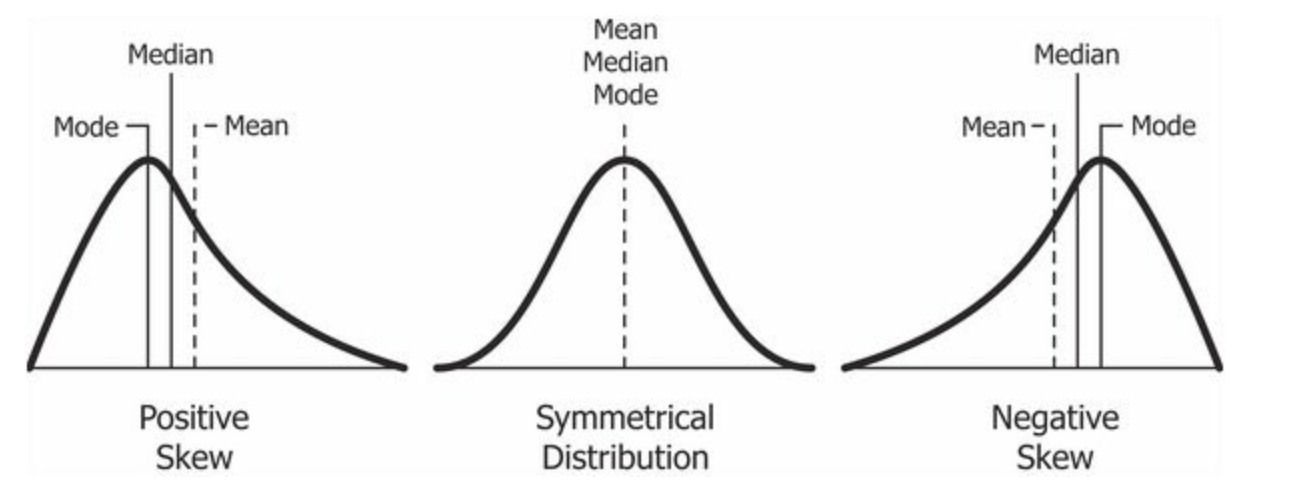
\includegraphics[width=3in]{skew.png}
\end{figure}

Since third powers are both positive and negative, skewness can be both positive and negative (and zero if the distribution is symmetric with right and left tails the same). 

In class, when we were looking at the normal DGP, we derived nonparametric MM estimators $\Xbar$ and $\sigsqhat$ for the expectation and variance (nonparametric meaning that the derivation for them was for all DGP's). Show that the nonparametric MM estimator for skewness is:

\beqn
\hat{\gamma} = \sqrt{n}\frac{\sum_{i=1}^n (X_i - \Xbar)^3
}{
\tothepow{\sum_{i=1}^n (X_i - \Xbar)^2}{3/2}
}
\eeqn

Hint: assume a iid DGP with density / mass function $f(\theta_1, \theta_2, \theta_3)$ where $\theta_1$ is the expectation, $\theta_2$ is the variance and $\theta_3$ is the skewness.
}\spc{15}


\end{enumerate}




\end{document}